% Applications, usage, collaborations.
% additional citations
   % ASMS?

% Sean's & Michael's comments on talk.
 
% Title and sig page to grad school
% Fall registration?

\documentclass[12pt,twoside,openright]{report}

\usepackage[margin=1in,inner=1.25in,includeheadfoot]{geometry}  % Set margins.
\usepackage{graphicx}              % Include graphics.
\usepackage{url}                   % Embed URLs.
\usepackage{multirow}              % Allow multi-row tables.
\usepackage{xspace}                % Add space at the end of a macro.
\usepackage{xr}                    % Allow cross-references between docs.
\usepackage[sort&compress]{natbib} % Hyphenate consecutive references.
\usepackage{setspace}
\usepackage{hyperref}

\author{{\Large Benjamin J. Diament}\\
\\
A dissertation submitted in partial fulfillment\\
of the requirements for the degree of\\
{\Large Doctor of Philosophy}\\
\\
University of Washington\\
\\
2011\\
\\
Program Authorized to Offer Degree:\\
Computer Science \& Engineering\\
}

\date{}

\newcommand{\XCorr}{\ensuremath{X_{Corr}}\xspace}
\newcommand{\Sp}{\ensuremath{S_p}\xspace}
\newcommand{\tidezero}{Tide-v0\xspace}
\renewcommand\contentsname{Table of Contents}

\title{Ultrafast and Real-Time Peptide Identification from Tandem Mass Spectra:
  Method and Applications}

\doublespacing

\let\origdoublepage\cleardoublepage
\newcommand{\clearemptydoublepage}{
  \clearpage{\pagestyle{empty}\origdoublepage}
}
\let\cleardoublepage\clearemptydoublepage

\pagestyle{empty}
\begin{document}

\maketitle

\cleardoublepage
\pagestyle{plain}
\setcounter{page}{1}
\pagenumbering{roman}
\tableofcontents

\newpage
\phantomsection \label{listoffig}
\addcontentsline{toc}{chapter}{List of Figures}
\listoffigures

\newpage
\phantomsection \label{listoftab}
\addcontentsline{toc}{chapter}{List of Tables}
\listoftables

\chapter{Preliminaries}
\pagestyle{myheadings}
\setcounter{page}{1}
\pagenumbering{arabic}

\section{Abstract}

Tide is a computer program that reimplements the SEQUEST method for identifying
peptides from tandem mass spectra. Employing a combination of algorithmic and
software engineering approaches, Tide's performance is hundreds to thousands of
times faster than SEQUEST's while retaining the exact same results as a recent
SEQUEST version.  One consequence of Tide is the possibility of peptide
identification in real time. We examine whether real-time peptide identification
can yield more unique IDs than the basic peak selection method can. We showed
that simple methods outperform the basic method only slightly, and that 
simulation has significant limitations in this context.

\section{Thesis Organization}

This thesis is organized into three parts. The first part is introductory.
Section~\ref{section:novelty} describes what is novel in this research and
the author's contributions. Section~\ref{section:background} reviews
background and terminology, and will be familiar to proteomics researchers.

The other two parts comprise the work of this thesis. Each part describes a
separate research project, with the second building upon the conclusions of the
first. The first project is the implementation of Tide, software for extremely
fast identification of peptides from tandem mass spectra using the SEQUEST
scoring method. This project tested the hypothesis that database search
according to the SEQUEST method could be made much faster by algorithmic means,
even while supporting a variety of complicating, but commonly-used, software
features. The second part of this thesis (Chapter~\ref{chapter:tide}) is an article, written jointly by myself and
Prof. Noble, describing Tide \cite{diament:faster}. The article was recently
published in the {\it Journal or Proteome Research}, and is reproduced here by
permission of the article's publisher.  Supplementary material published along
with that article is included here as well, and gives details on the specific
algorithms and strategies used in Tide.

The second research project was the simulation of various procedures for
ID-informed peak selection (IDIPS) in the context of real-time peptide
identification. (These terms are defined in Sections~\ref{section:background}
and \ref{chapter:realtime}). This project tested the hypothesis that IDIPS can
yield significantly better peptide identifications -- as measured by the number
of distinct peptides identified -- than the basic peak selection method
does. The third part of this thesis, Chapter~\ref{chapter:realtime}, describes
our research in real-time peptide identification and ID-informed peak selection.

\section{Novel Aspect and Author's Contributions}
\label{section:novelty}

Tide is the peptide identification software that I wrote. Tide was built upon the
peptide identification methodology and scoring function originally pioneered
with SEQUEST and further developed in Crux, which introduced a peptide index to
improve search speed. No aspect of the scoring function in Tide is novel.

My novel contribution through Tide was a further thousandfold (in several test
cases) speed improvement over Crux and SEQUEST by means of algorithmic and
software engineering techniques. There was no {\it a priori} guarantee that any
substantial further speed improvements (beyond Crux's) would have been
possible. This first part of my research has been the most successful in
achieving its aims.

I furthered my original work on Tide by adding an array of features which are
standard for software of this type (including SEQUEST, Crux, and most other
peptide search software). Most significantly, I added support for searching
peptides with variable modifications. My original contribution in so doing was
to show (in the face of some expressed doubt) that Tide's speedup could be
maintained (and in some cases exceeded) in the context of variable modification
search. As a caveat, however, this feature is implemented in a way that often
results in extremely high disk usage, which may detract from its utility in some
cases. I have not undertaken to mitigate this effect, and doing so is beyond
the scope of my thesis.

I have shown Tide's utility in real proteomics research in two contexts. I
helped facilitate the use of Tide in a large-scale project in which executing a
search using SEQUEST would have been very costly. This project was a reanalysis
of 15 years of spectrometry experiments from the Yeast Resource Center. I also
examined the applicability of Tide to another project: a collection of
experiments from the Global Ocean Survey analyzed originally over the course of
a month on an 800-core compute cluster in the Goodlett Laboratory, Department of
Medicinal Chemistry, University of Washington. The data consisted of $\sim
400,000$ MS/MS spectra searched against a $6.1$ million-protein database,
yielding $235.8$ million peptides, including modified forms. Experiments show that
Tide would take about 17 hours on a single thread of a single machine to do the
equivalent computation.

I realized that the prospect of a thousandfold speed improvement in peptide
identification suggested the possibility of using identifications in real time
to drive the spectrometer's peak selection algorithm adaptively (see
Sections~\ref{section:background} and \ref{section:adaptivepeak}). I
worked with Prof. Noble to flesh out the idea. Prof. Noble suggested the method
for collecting simulation data and wrote the original tool for assembling it
(see Section~\ref{subsection:simulationdata}). I developed and implemented
the simulation methodology and ran the experiments. Together, Prof. Noble and I
developed several peak selection procedures and the means to evaluate them.

\section{Background}
\label{section:background}

Shotgun proteomics using tandem mass spectrometry (MS/MS) is devoted to the
characterization of proteins in a laboratory sample. Its aim is to identify the
chemical makeup of each protein in the sample and the quantity of each
protein. The makeup of such proteins is not arbitrary; having been generated by
a living organism, the sample must comprise only proteins that the organism can
produce. The full library of proteins is known nearly completely for a number of
different species, from bacteria to human, and is known partially for
others. The field of genomics has recently engendered explosive growth in the
availability and comprehensiveness of protein databases, as the mapping from
genome to proteome is fairly well understood.

In rough summary, a typical shotgun proteomics experiment proceeds as follows
\cite{steen:abcs}: a protein sample, adequately separated and purified by
chemical means, is digested by the enzyme trypsin. The digest is subjected to
liquid chromatography (LC) and slowly fed, over the course of 30 minutes to
three hours, into a tandem mass spectrometer, which analyzes a small amount of
the substrate at frequent intervals, making about 5--10 measurements per second.

The tandem mass spectrometer operates in two stages, alternating one detailed
{\it MS1} scan with about 5--10 less-detailed {\it MS/MS} scans per duty
cycle. The on-board computer records the {\it retention time} at which the scan
is taken, which corresponds to the hydrophobicity of the peptides then eluting
off the LC column. Many thousands of peptide species may elute over the course
of a spectrometry run. The chromatographic separation is performed in order to
group the peptides by hydrophobicity so that a smaller number of peptide species
may appear in any given scan, greatly simplifying the analysis.

Each scan taken by the spectrometer gives a measurement for each $m/z$ value
corresponding to the number of times the instrument counted a particle with that
mass-to-charge ratio. The measurement is called the {\it intensity} at that
$m/z$.  Because there are a substantially smaller number of particle types
eluting at one time than there are possible $m/z$ values at which the
spectrometer can take a measurement, the intensity at most $m/z$ values is zero
(ignoring the considerable influence of chemical and electrical
noise). Consequently, only a sparse set of $m/z$ values at have a positive
intensity. Because of this sparsity, at those $m/z$ values where the intensity
is nonzero, there is said to be a {\it peak}.

Both the MS1 and MS/MS scans measure the masses of the particles eluting off the
LC column at a given time, but MS1 measures intact peptides across a wide
mass/charge ($m/z$) range (typically covering 1000 $m/z$), whereas MS/MS
measures a fragmented peptide isolated from a narrow $m/z$ range (typically a
fraction of one $m/z$). The fragments are then measured across the full $m/z$
range. Thus the data associated with an MS/MS scan is:
\begin{enumerate}
\item the retention time at which the scan was taken,
\item the $m/z$ value of the window from which the peptide was isolated (the
  {\it precursor} $m/z$), and
\item the set of ($m/z$, intensity) values of the peaks in the scan.
\end{enumerate}

The $m$ value, measured in Daltons, is simply the mass of the peptide or
fragment, which may be theoretically determined by summing the masses of the
amino acids in a peptide's or fragment's amino acid sequence. This mass is the
number that is needed for analysis. However, the spectrometer actually outputs a
mass/charge ($m/z$) ratio, where the charge $z$ is a small integer (1, 2, or 3,
for our purposes) whose value is unknown {\it a priori}. Whatever the charge of
the precursor, however, the charge of the fragments cannot be higher. For our
purposes, the charge is merely a confounding factor: it serves no function, but
we need to be aware of the charge in determining what mass a peptide or fragment
may have.

The goal of the full shotgun spectrometry experiment is to identify as many
distinct peptide species as possible as present in the sample. With each MS1
scan, the spectrometer's on-board computer must select a subset of peaks to
isolate, fragment, and measure in an MS/MS scan. In each duty cycle, hundreds of
MS1 peaks may be reasonable candidates for MS/MS analysis, but the available
time permits only a small fixed number (5--10) to be analyzed, so only a
fraction of these will be identified. In order to maximize the number of
distinct peptides analyzed, the peaks are typically selected by highest
intensity, subject to a strategy intended to diversify the set of peptides
examined. In the last portion of this thesis, where it plays a central role, we
discuss peak selection in more detail.

After the spectrometry experiment finishes, analysis software examines the
precursor mass and fragment masses, and identifies a peptide sequence that best
accounts for the MS/MS data. A vast collection of software exists for
identifying tandem mass spectra \cite{nesvizhskii:analysis}. We discuss various
software approaches and techniques, along with other relevant background in more
detail in Section~\ref{section:tideintro}.

\input{tide}
\documentclass[12pt]{article}

\usepackage[margin=1in]{geometry}  % Set margins.
\usepackage{graphicx}              % Include graphics.
\usepackage{url}                   % Embed URLs.
\usepackage{multirow}              % Allow multi-row tables.
\usepackage{xspace}                % Add space at the end of a macro.
\usepackage{xr}                    % Allow cross-references between docs.
\usepackage[sort&compress]{natbib} % Hyphenate consecutive references.
\usepackage{setspace}

\author{Benjamin Diament\\
Department of Computer Science and Engineering\\
University of Washington\\
Seattle, WA, USA\\
bdiament@cs.washington.edu
\and
William Stafford Noble
\thanks{
to whom correspondence should be addressed.
email: william-noble@uw.edu;
phone: 206-543-4457;
fax: 206-685-7301
}\\
Department of Genome Sciences\\
Department of Computer Science and Engineering\\
University of Washington\\
Seattle, WA, USA\\
william-noble@uw.edu}

\newcommand{\XCorr}{\ensuremath{X_{Corr}}\xspace}
\newcommand{\Sp}{\ensuremath{S_p}\xspace}
\newcommand{\tidezero}{Tide-v0\xspace}



% Allow references to the main document.
\externaldocument{tide}

\usepackage{float}
\floatstyle{plain}
\newfloat{suppfigure}{p}{cap}
\floatname{suppfigure}{Supplementary Figure}

\title{Supplement to ``Faster SEQUEST Searching for Peptide
  Identification from Tandem Mass Spectra''}

\begin{document}

\maketitle

The following sections describing Tide's major speed enhancements
are organized topically and not strictly in the order the improvements
were introduced. Decisions on that progression were made
incrementally, after evaluating the timing and profile following each
change. Consequently, it is impossible in some cases to determine
the performance improvement due to each of these changes
individually. Moreover, some of the later optimizations intrinsically
rely on earlier ones. For instance, making the theoretical peak set
five-fold sparser (Section~\ref{subsubsection:fivefold}) cannot happen
without the sparse peak representation
(Section~\ref{subsubsection:sparsepeaks}), and run-time compilation of the
dot-product code (Section~\ref{subsubsection:compiler}) requires the FIFO
memory allocation scheme (Section~\ref{subsubsection:fifo}).

Each of the following subsections describes a technique Tide uses to
gain performance.

\section{Sparse Representation of Theoretical Peaks \label{subsubsection:sparsepeaks}}

Each peptide's theoretical spectrum consists of ten peaks for each
amino acid in the peptide, for each charge state, corresponding to the
major ion types and the related neutral losses. Since there are
roughly 1,000 mass/charge buckets (depending on machine settings), and
since most peptides are short (under 20 amino acids), the theoretical
spectrum is typically sparse, so Tide uses a sparse representation of
the theoretical peaks. This change enabled another technique---making
theoretical peaks five-fold sparser (Section~\ref{subsubsection:fivefold}).

\section{Heapify to find Top Matches}

As Crux finds candidate peptide-spectrum matches, it adds them to an
array, which it sorts to find the best five matches. In place
of this sort, Tide uses a heapify operation which requires linear time
rather than the $O(n \log(n))$ time required by the sort to find the top
matches.

\section{Linearizing Background Subtraction \label{subsubsection:linearize-bkgnd-sub}}

SEQUEST's original implementation, and the first Crux implementation
of \XCorr, take the sum, over all $i$, of the expression:
\[
\mbox{\XCorr}_i(u,v)=u_iv_i-\frac{1}{150}\sum_{\tau=-75}^{75}{v_iu_{i-\tau}}
\]
where
\[\frac{1}{150}\sum_{\tau=-75}^{75}{v_iu_{i-\tau}}\]
is the ``background'' at the $i$th vector position. It was pointed
out in \cite{eng:fast} that this computation could be sped up by
pulling the $v_i$ out of the sum, and subtracting the background from the
observed spectrum before computing a dot product with each candidate
theoretical spectrum $v$. That is, one could compute the equivalent
expression
\[
\XCorr(u,v)=\sum_{i=1}^{N}{v_i\left[u_i-\frac{1}{150}\sum_{\tau=-75}^{75}{u_{i-\tau}}\right]}
\]
The bracketed portion need be computed only once. This improvement
already existed in Crux and in \tidezero. However, Crux performs the
background subtraction (the bracketed sub-expression above for each
index i) using a double loop as follows:

\begin{verbatim}
For each bin's value b in the bucketed observed spectrum:
  For each bin w in the 150-bin window surrounding b:
    b -= w/150
\end{verbatim}

In Tide, this double loop is linearized by first computing the array
of partial sums roughly according to the following pseudocode. (The
edge cases and array initializations are omitted for clarity):

\begin{verbatim}
For integer i ranging over the array of bins:
  partial_sums[i] = partial_sums[i-1] + bin[i]

For integer i ranging over the array of bins:
  bin[i] -= (partial_sums[i+75] - partial_sums[i-76])/150
\end{verbatim}

At the stage it was introduced, this speedup reduced the total running
time by about 47\% (see line 5 in Table~\ref{table:timing}).
Figure~\ref{figure:profiles}(b) shows profiles just before and after this
change: the background subtraction loop had been occupying most of the
spectrum preprocessing time.

Following this change, on benchmark datasets tested, spectrum
preprocessing occupied surprisingly little of the total run time, even
though it has not otherwise been optimized. The relatively low cost of
spectrum preprocessing is due mostly to the large number of peptide
candidates per spectrum. The main consequence of this relatively low
cost is that it was usually correct to move as many computations as
possible from computing theoretical peaks and the dot product to the
spectrum preprocessing stage.

\section{Caching Multiplications}

Crux and \tidezero computed the dot product of each observed spectrum
with each candidate theoretical spectrum. \tidezero did so in a
straightforward manner with a single multiplication and addition at
each bucket. However, each of the theoretical peaks may have one of
only three possible intensities: 10, 25 or 50. The common case is that
there are many candidate peptides for each observed spectrum, so it
pays to scale the observed spectrum by each of these factors and to
cache the results. An array, {\tt peaks}, of the original values is
stored and then three caches, {\tt peaks10}, {\tt peaks25}, and
{\tt peaks50} are computed before iterating over the candidate
peptides. For each candidate peptide, the dot product is performed by
simply looking up the correct cache entry, and adding the correct
entries together. This eliminates the multiplications during dot
product computation.

To accommodate this change, the theoretical spectra are represented as
a sparse vector of pairs {\tt (scalar\_enum, bucket)} where
{\tt scalar\_enum} is an enumeration:
\begin{verbatim}
enum { Peaks10 = 1; Peaks25 = 2; Peaks50 = 3; }
\end{verbatim}
indicating which scaled cache to use, and bucket indicates the correct
entry in the scaled cache.

The dot product loop then requires two array lookups and an addition
per theoretical peak:
\begin{verbatim}
dot_prod += cache[scalar_enum][bucket];
\end{verbatim}

\section{Array Striping \label{subsubsection:striping}}

The dot-product code above was further improved by interleaving (striping) the
three cache arrays together, eliminating one of the memory lookups in the tight
dot-product loop above. This is possible even though the extent of the observed
spectrum is not known at the time the theoretical spectrum is computed. At the
time this change was introduced, performance improved by about 17\%, as shown in
line 10 of Table~\ref{table:timing}.

\section{Join with Rolling Window \label{subsubsection:join}}

\begin{figure}
\centering
\includegraphics[width=6.0in]{Diagrams_p2-p2-cropped.pdf}
\caption{{\bf Data flow after introducing the rolling window join}
  \label{figure:join}}
\end{figure}

Crux implements an index, not present in early versions of SEQUEST,
containing all input peptides sorted by precursor mass. As each
spectrum in the input file is received, Crux seeks to the beginning of
a user defined window around the precursor mass. Then it computes the
theoretical spectrum for each peptide in that window, comparing each
successively in turn against the observed spectrum from the input. Two
significant downsides remain in this approach: there is a call to the
{\tt seek()} function 
per spectrum, and the same theoretical spectrum may be recomputed many
times over the course of a run. \tidezero did not suffer the disk seek
problem, but only because it allowed peptide sets of only very limited
size and kept them in memory.

The rolling-window join, described presently, eliminates the call to 
the {\tt seek()} function
without requiring that the whole index reside in memory, and it
eliminates significant recomputation of theoretical spectra. As
SEQUEST, Crux, and \tidezero were structured, the same theoretical
peak set is recomputed from a peptide whenever the peptide is a
candidate match for two different spectra. Rather than recompute
these, Tide creates opportunities for theoretical spectra to be reused
when possible.  To do this, Tide employs a ``rolling window'' join of
sorted peptides against sorted observed spectra.

Two changes are implemented. First, before any matching begins, all
the observed spectra are read into memory and sorted by mass.  In case
a spectrum has multiple possible charge states it appears in the
sorted array once for each charge state, as the join is performed on
the neutral (uncharged) mass.

Critics will note that reading all spectra into memory at the start is
not scalable to large sets of spectra. However, it is of much less
concern to read the spectra into memory than the candidate peptides,
since there are, for most uses, many fewer spectra than
peptides. Represented compactly, spectra can occupy about 500-1000
bytes each. Once a spectrum is evaluated, it can be discarded
completely. This suggests the following scheme as Tide scales, if
memory becomes saturated by reading in the spectra at once: at the
sorting step, one could sort spectra in batches, store to disk, and
merge the files as they were re-read as input to the join. Because Tide
is CPU-bound, disk-based costs of doing this merge could be managed by
threading. All of this is independent of the join method itself.

After the spectra are sorted, the join is performed as follows. Tide
iterates over the spectra sorted by neutral mass. At the same time,
Tide reads the presorted candidate peptides into an ``active peptide
queue.'' The queue contains just the peptides that fall within the
user-specified precursor mass window. As Tide iterates over each
successive observed spectrum, it evicts from the queue and discards
any candidate peptides whose masses are too small for the current observed
spectrum. Then Tide reads from the presorted peptide index, enqueueing
each, until it arrives at the first peptide that is too massive. This
last peptide is placed in the queue but does not fall within the
active window. The queue must support not only the standard enqueue
and dequeue operations, but also allow iteration over its contents
(without altering them). Iteration over the queue contents creates a
``rolling window,'' which occupies only as much memory as is required
to store a window's worth of theoretical spectra. This enables reuse
of the computation of the theoretical spectra so that no theoretical
spectrum need ever be computed more than once. No explicit call to the 
{\tt seek()} function
is ever performed.

At the stage it was implemented, this change cut Tide's running time
by 64\%, as shown in line 6 of Table~\ref{table:timing}. The changes
to the data flow of Tide, following the introduction of the rolling
window, are shown in Figure~\ref{figure:dataflow}(B).

\section{
  Making the Theoretical Peaks Vector Five-fold Sparser
  \label{subsubsection:fivefold}
}

Theoretical spectra in the SEQUEST algorithm occur in groups
corresponding to cleavage events, with somewhat predictable spacing
among the peaks within a group. It is possible to take advantage of
such peak groupings to represent the complete set of theoretical peaks
even more sparsely.

As explained above, the theoretical peaks vector includes ten peaks
per amino acid: the $b$-ion and $y$-ion, each with intensity 50; the
two bins flanking each of the $b$- and $y$-ions, each with intensity
25 (four peaks total); the neutral loss of ammonia for each $b$- and
$y$-ion, each with intensity 10 (two peaks); the neutral loss of water
from each $b$-ion with intensity 10; and the $a$-ion with intensity
10. The same pattern is repeated for all the ions of charge two.

Importantly, the position of some of these ions is fixed relative
to the positions of some others. This is not always true, but it is
approximately so:
\begin{enumerate}
\item The flanking ions around each of the $b$- and $y$-ions are always
  one bin away on either side.
\item The peak for the neutral loss of ammonia is usually 17 bins away
  from the corresponding $b$- and $y$-ions, but is occasionally (0.014\%
  of the time) 18 bins away. For charge-2 ions, the neutral loss of
  ammonia is either at 8 or 9 bins away, about half the time at each.
\item The peak for the neutral loss of water is usually 18 bins away
  from the corresponding $b$-ion, but is occasionally (0.0015\% of the
  time) 19 bins away. For charge-2 %b%-ions, the neutral loss of water is
  either usually at 9 bins away, but occasionally (0.46\% of the time)
  10 bins away.
\item The peak for the $a$-ion is usually 28 bins away from the
  corresponding $b$-ion, but is sometimes (0.014\% of the time) 27 bins
  away. For charge-2 ions, the corresponding $a$-ion is usually at 14
  bins away, but 8.6\% of the time is 13 bins away.
\end{enumerate}
These observations suggests the following optimization, which is implemented in
Tide. Rather than compute all ten (or 20 for charge-2) peaks for each
amino acid in each peptide, we compute only the $b$- and $y$-ion. At the
time of spectrum preprocessing, we compute a larger cache, consisting
not only of the scaled vectors Peak10, Peak25, and Peak50 but also the
following new vectors:
\begin{verbatim}
PeakY1[i] = Peak50[i] + Peak25[i-1] + Peak25[i+1] + Peak10[i-17];
PeakB1[i] = PeakY1[i] + Peak10[i-18] + Peak10[i-28];
\end{verbatim}
These vectors represent the relative positions of the peaks that get added
together as we take dot products in most cases. Similar cache vectors
are computed for the charge-2 versions in each of the two forms where
ammonia is 8 or 9 bins away.

With these cached values, a theoretical vector five times sparser than
before may be used to compute the dot product. However, some bins
will be wrong for some peptides, because the neutral-loss peaks
are not always the same distance from the $b$- and $y$-ions. Therefore,
for each theoretical spectrum we compute the very sparse vector, $s$,
of just $b$- and $y$-ions and we separately compute the original sparse
vector of peaks, $r$, which gives the correct calculations, and then
take the difference $r-s \equiv d$. Because $r$ and $s$ are often the same, $d$ is
often empty, and when not, is very sparse. By computing $s$, $r$, and $d =
r-s$, for each theoretical spectrum we can compute the dot product:
$\langle u,s \rangle + \langle u,d\rangle$ in place of $\langle u,r
\rangle$ where $u$ is the observed spectrum.

At first, applying this heuristic led to almost no observable change in performance (see line 9
of Table~\ref{table:timing}); however, the profile as shown in
Figure~\ref{figure:profiles}(c) shifted: the largest consumer of time
is no longer the dot product, but rather the computation of $d$. This
is an improvement, since the computation of $d$ has not been optimized
at this point. In fact, optimizing the computation of $d$ is not
necessary: $d$ is so sparse that it is profitable simply to
precompute it at indexing time, store it to disk and read it back
with each peptide. Line 11 of Table~\ref{table:timing} shows the 24\%
savings when $d$ gets precomputed and stored to disk.

\section{Fixed Point Arithmetic \label{subsubsection:fixedpoint}}

Another performance change breaks, albeit very slightly, the aim to
preserve exactly the output of Crux. Rather than compute the dot
product in double-precision floating-point arithmetic, Tide uses
fixed-point arithmetic. This approach is possible only because the
normalization procedure applied to the observed spectrum greatly
constrains the range of values of the intensities. To do this, Tide
multiplies each entry in the spectrum by a large constant ($10^7$) and
rounds to the nearest integer. The constraints imposed by the
normalization procedure ensure against underflow or overflow, and the
fact that the dot product is a simple summation assures numerical
stability. We therefore achieve the same results as Crux does to at
least five or six decimal places. Because of \XCorr's instability, as
mentioned above, this precision is far beyond where \XCorr values
remain meaningful. The effects of this change, however, were small on
the benchmark sets, and it remains unclear whether this change
helps. See line 12 of Table~\ref{table:timing}.

\section{FIFO Memory Allocator \label{subsubsection:fifo}}

Further profiling of a larger dataset showed that significant time
was still being spent in memory heap operations, many of which were
tied to allocating and deallocating space for theoretical spectra and
associated data.

The built-in memory allocator typical of most C and C++ programs makes
no assumptions on the order in which blocks of memory will be
allocated and deallocated. It therefore needs to keep careful track of
which blocks of memory are in use at any given time. Updating this
information as a program runs can take significant time in case many
allocation and deallocation operations are performed, as is the case
in Tide. However, in Tide, the pattern of allocations and
deallocations closely mirrors the enqueuing and dequeueing of
candidates in the active peptide queue, described in
Section~\ref{subsubsection:join}. This first-in-first-out (FIFO)
memory usage pattern is entirely predictable: if memory block $A$ is
allocated before memory block $B$, then $A$ will be freed before
$B$. This greatly simplifies the bookkeeping usually associated with
the built-in memory allocator such that the memory needed by Tide can,
for the most part, be kept in a contiguous region of machine
memory. Therefore, we introduced in Tide a specialized
first-in-first-out memory allocator that performs well on data
allocated according to the FIFO usage pattern.

\section{Compiled Dot-Product Code \label{subsubsection:compiler}}

Following the above speed improvements, profiling revealed that most
of the remaining time (about $60\%$) was spent in the dot product
computation:
\begin{verbatim}
for (int i = 0; i < num_theoretical_peaks; ++i)
  total += cache[theoretical_peaks[i]]
\end{verbatim}

This loop was already improved twice, using cache lookups instead of
multiplication operations, and using two such lookups rather than
three. Still, testing showed that unrolling this loop and hard-coding
specific values for the {\tt theoretical\_peaks} array was about twice
as fast. To illustrate the difference, suppose
{\tt theoretical\_peaks} contained these values:
{\tt 171,226,229,232,525},\ldots, etc.
Then tests showed it was roughly twice as fast as the above dot
product loop to execute:
\begin{verbatim}
total = cache[171] + cache[226] + cache[229] + cache[232] + cache[525] + ...
\end{verbatim}
The speedup is likely due to executing one less memory lookup per
array entry. But the specific values in {\tt theoretical\_peaks} are
unavailable until the theoretical peak set is computed at run
time. However, the same theoretical peak set may be reused many times.

To take advantage of this, Tide performs a run-time compilation for
each theoretical spectrum to {\tt x86} machine code to execute the
sum with preset values. The appropriate code is generated in a buffer
for each candidate peptide and the program is instructed to jump to
the buffer to run this peptide-specific dot-product code. The overall
savings is shown in line 13 of Table~\ref{table:timing}.

\bibliographystyle{unsrt}
\bibliography{refs}

\end{document}


\chapter{Real-Time Peptide Identification and ID-Informed Peak Selection}
\label{chapter:realtime}

We now reconsider the question of how MS1 peaks are selected for fragmentation
and analysis in a shotgun proteomics experiment, first discussed in
Section~\ref{section:background}. Until now, MS1 scans have been the only
real-time source of information on which the spectrometer's on-board computer
could reasonably draw to make decisions about which peaks to choose for
fragmentation. However, the introduction of Tide shows that high-speed
identification of MS/MS scans by searching a peptide database is possible. This
possibility raises the following question: Could we identify MS/MS spectra as
they are acquired in real time, and could we then use this information to
improve the peak selection strategy employed by the on-board computer?

We introduce the term {\it ID-informed peak selection} ({\it IDIPS}) to mean
choosing peaks not solely on the basis of MS1 data, but also on the basis of
MS/MS peptide identifications that have been made in real time. Previously,
instrument manufacturers were not able to make use of real-time peptide
identification based on database search because sufficiently fast technology had
not been available. This is the reason that the basic exclusion list uses MS1
information only.

The central hypothesis of this portion of the thesis is that ID-informed peak
selection (IDIPS) will yield significantly better peptide identifications -- as
measured by the number of distinct peptides identified -- than the basic
exclusion list does. A sampling of some IDIPS strategies and their performance
under simulation is the main experimental result of this part of this thesis.

\section{Real-Time Peptide Identification}
\label{section:lowlatency}

In order to perform ID-informed peak selection, we need a system that can do three
things, of which a typical peptide database search program can do only the
first:

\begin{enumerate}
\item perform a database search of reasonable complexity,
\item achieve high bandwidth on a single computer, and
\item achieve low latency between spectrum acquisition and identification.
\end{enumerate}

To achieve reasonable search complexity for a typical shotgun proteomics
experiment, we want to be able to search a database of proteins from a single
target organism, plus contaminants, with some reasonable settings, such as a
semi-tryptic digest and a sufficiently wide precursor tolerance
window. Reasonable database size, digest, and tolerance window are significant
contributors to search time. All modern peptide search software, including Tide,
can perform reasonably complex searches.

Tide is also able to achieve high bandwidth on a single computer, as shown in
the first part of this thesis. However, the current implementation of Tide
assumes that all spectra to be searched are available at the start of
computation. This assumption, while reasonable in the context of most proteomics
laboratory pipelines, fails in the context of real-time peptide identification.

To achieve ID-informed peak selection, we need to identify spectra in time to
make on-the-fly decisions on which peaks to select for fragmentation. We
therefore need to a low-latency peptide identification method, meaning that
spectra are identified within a very short time (say, a few seconds) after the
spectrum has been acquired. This requirement is distinct from that of high
bandwidth, though the two requirements are related and can be addressed using
many of the same approaches.

Tide begins processing by sorting the input spectra by neutral mass, which is
required for the rolling window join (Section~\ref{section:join}). A
low-latency version of Tide would not be able to access all spectra at the start
of processing, and hence cannot perform the rolling window join. Some
alternative is required, and we discuss this next.

The rolling window join achieves two important objectives: reusing the
computation of the theoretical spectrum and maintaining a small memory footprint
over the course of computation. The first objective is critical for speed, and
some alternative implementation is required to achieve the same level of
performance. The second objective -- maintaining a small memory footprint -- is
of intermediate importance: there needs to be sufficient memory available to
complete the computation, but there is no need to conserve beyond that point.

\section{Adapting Tide for Real-Time Computation}

A simple substitute strategy for the rolling window join is to preload all
theoretical spectra in memory in advance of collecting the first
spectrum. Before any spectrum is preprocessed, the index of candidate peptides
is loaded from disk, and the programs generated by the run-time dot-product code
are all compiled at that time, exactly as described in
Section~\ref{section:compiler}. However, these dot-product programs are all
retained in memory and not released, as they would be in the rolling-window-join
procedure.

The preloading approach has the potential for enormous impact on the program's
memory usage, but it also leaves the total running time (including the
preloading step) almost exactly the same as for the current Tide. This approach
maintains the guarantee that each theoretical spectrum will be computed at most
once, at program startup. Thereafter, the theoretical spectra will not have to
be recomputed at all. All the functions of Tide are performed under the
preloading approach, but in a different order than for Tide. Except for the
larger memory footprint, the resource usage does not change.

We now address the question of whether enough memory would be available to
perform a reasonable peptide identification experiment under the preloading
strategy. We first measure empirically how much memory would be consumed. The
current implementation of Tide interleaves the preprocessing of the observed
spectra, the computation of the theoretical spectra, and computing the
\XCorr. The interleaving allows us to free memory used by the theoretical
spectrum computation once the relevant candidate peptides are no longer
needed. If we do not free the corresponding memory, then we can measure how much
memory would be used by the alternative approach described.

\begin{figure}
\centering
\includegraphics[width=6.0in]{mem_footprint.pdf}
\caption[Disk and Memory Footprint for Preloaded Theoretical Spectra]{{\bf Disk
    and Memory Footprint for Preloaded Theoretical Spectra.} For each of four
  benchmark data sets, the size of the index on disk is shown. We also show the
  cumulative amount of memory allocated during processing (ignoring
  deallocations) for each benchmark. This shows an upper bound on the memory
  required to preload the machine with all theoretical spectra.
  \label{figure:footprints}}
\end{figure}

Figure~\ref{figure:footprints} shows the total disk usage and cumulative memory
allocated (ignoring reuse) by Tide when run in each of four modes. We see that
the worm dataset, which needs the larger database requires more memory than
yeast under comparable settings. We also see that semi-tryptic digestion is
considerably more memory-intensive than fully-enzymatic digestion. Even in the
most intensive case, only 6GB of memory is allocated in total. These results
show that on a modern workstation, there is sufficient memory not only for a
fully tryptic search, but even for a substantially larger semi-tryptic search,
even without substantial changes to data structures.

Much larger searches, such as non-enzymatic digest or searches allowing multiple
modifications per peptide, would require more memory and more time than the
above strategy provides. There certainly remain limits to what can be achieved
in a real-time context, but the foregoing discussion brings closer together the
notions of high-throughput and of real-time peptide identification.

We have not implemented a low-latency version of Tide according to the method
described here. We opted first to perform simulations to ascertain the
feasibility of ID-informed peak selection. Had we seen more positive results from
testing, a low-latency implementation of Tide would be the next step.

\section{Adaptive Peak Selection} %%2
\label{section:adaptivepeak}

\subsection{Basic Exclusion List}

Peak selection is the process by which a spectrometer uses MS1 data and its own
operational history over the course of a run to choose which $m/z$ values will
be isolated and subjected to fragmentation and MS/MS. Over the course of a
tandem mass spectrometry run, MS1 scans are collected every second or so,
roughly once for each 5-10 MS/MS spectra. Each MS1 spectrum indicates the peak
intensity for each unfragmented peptide at a specific retention time and
mass/charge ($m/z$) ratio. The peak intensities as a function of $m/z$ can be
used as a proxy for peptide abundance, and may be used to select an $m/z$ window
for subsequent fragmentation.

The spectrometer's on-board computer is responsible for deciding which peaks
will be selected for fragmentation at each duty cycle consisting of an MS1 scan
and multiple corresponding MS/MS scans.  This on-board computer uses an {\it
  exclusion list} to manage peak selection. The main goal of the exclusion list
protocol is to maximize the number of distinct peptides identified. The
exclusion list uses a two-part approach to achieve this. First, it aims to
gather spectra principally from abundant peptides, which are likely to be of
higher quality and hence easier to identify.  Second, the exclusion list aims
for a diverse set of peptide species to be chosen. Taken together, these goals
are intended to lead to a broad sampling across abundant peptides in the sample.

Before we describe the workings of the basic exclusion list, we note that its
two approaches are at odds with each other. If the only goal were to gather
abundant peptides, we could simply repeatedly sample the abundant peaks, but we
wouldn't see much diversity. On the other hand, if we sampled randomly across
all peaks regardless of abundance, we would get diversity without regard to
abundance, and we would also expect to see more spectra of poor quality, because
of low signal-to-noise ratio.

The standard exclusion list works as follows. A list of maximum fixed size
(about 50) of $m/z$ values is maintained in the on-board computer's memory and
is initialized to be empty. With each MS1 scan, the highest-intensity peaks are
examined in order. Any peak already on the exclusion list is ignored. Any peak
not on the exclusion list is selected for fragmentation and is placed on the
exclusion list. This process continues until 5 peaks have been selected for
fragmentation. Once a peak is placed on the exclusion list, it remains there for
a user-specifiable period of time, typically around 30 seconds.

\subsection{ID-Informed Peak Selection}

A real-time implementation of Tide offers the possibility of ID-informed peak
selection (IDIPS), as defined above. The term IDIPS does not name a specific
strategy for using the available real-time peptide identifications, but refers
to any such strategy.

Naturally, over the course of a spectrometry run, we only have access to MS1 and
MS/MS data that were collected at earlier points in the experiment, so any
realistic peak selection strategy may reasonably make use only of those MS/MS
scans that occurred prior to the current MS1 scan. We do, however, envision the
possibility of a slight delay (latency) separating the acquisition of the MS/MS
spectrum from its identification. In that case, the peak selection strategy may
only refer to MS/MS scans that were completed earlier by an amount of time equal
to the latency.

\subsection{Peak Selection Procedures}

A {\it peak selection procedure} is any specific procedure that operates in the
framework of IDIPS to choose individual MS1 peaks for
fragmentation at each time point. The procedure may refer to current and past
MS1 data, as well as MS/MS identifications corresponding to peaks previously
selected. The selection procedure is separate from simulation, identification
and evaluation.

As introduced above, our hypothesis is that adaptive peak selection done
according to some ID-informed peak selection procedure will yield better peptide
identifications over the course of a spectrometry experiment. We now turn to
describing how we tested this hypothesis.

\section{Simulation} %%3

Before attempting to implement IDIPS on a real experiment, we
wanted to prove the concept first. To this end, we simulated the action of a
spectrometer able to select peaks adaptively. In the simulation, the
spectrometer has access to real-time peptide identifications as they would be
performed by a real-time Tide implementation and is able accordingly to select
peaks for fragmentation.

The simulator works in conjunction with a given experimental peak-selection
procedure, which we evaluate as an alternative to the basic exclusion list. The
same simulator is used in conjunction with a variety of peak-selection
procedures, and is coupled with these procedures one at a time for
evaluation. We tested thousands of these procedures, grouped by overall strategy
and corresponding parameters.

The simulator and peak selection algorithm work together with Tide and an
evaluator module that simply counts how many peptides were identified in the
simulated run. The simulation framework is diagrammed in
Figure~\ref{figure:simulator}.

\begin{figure}
\centering
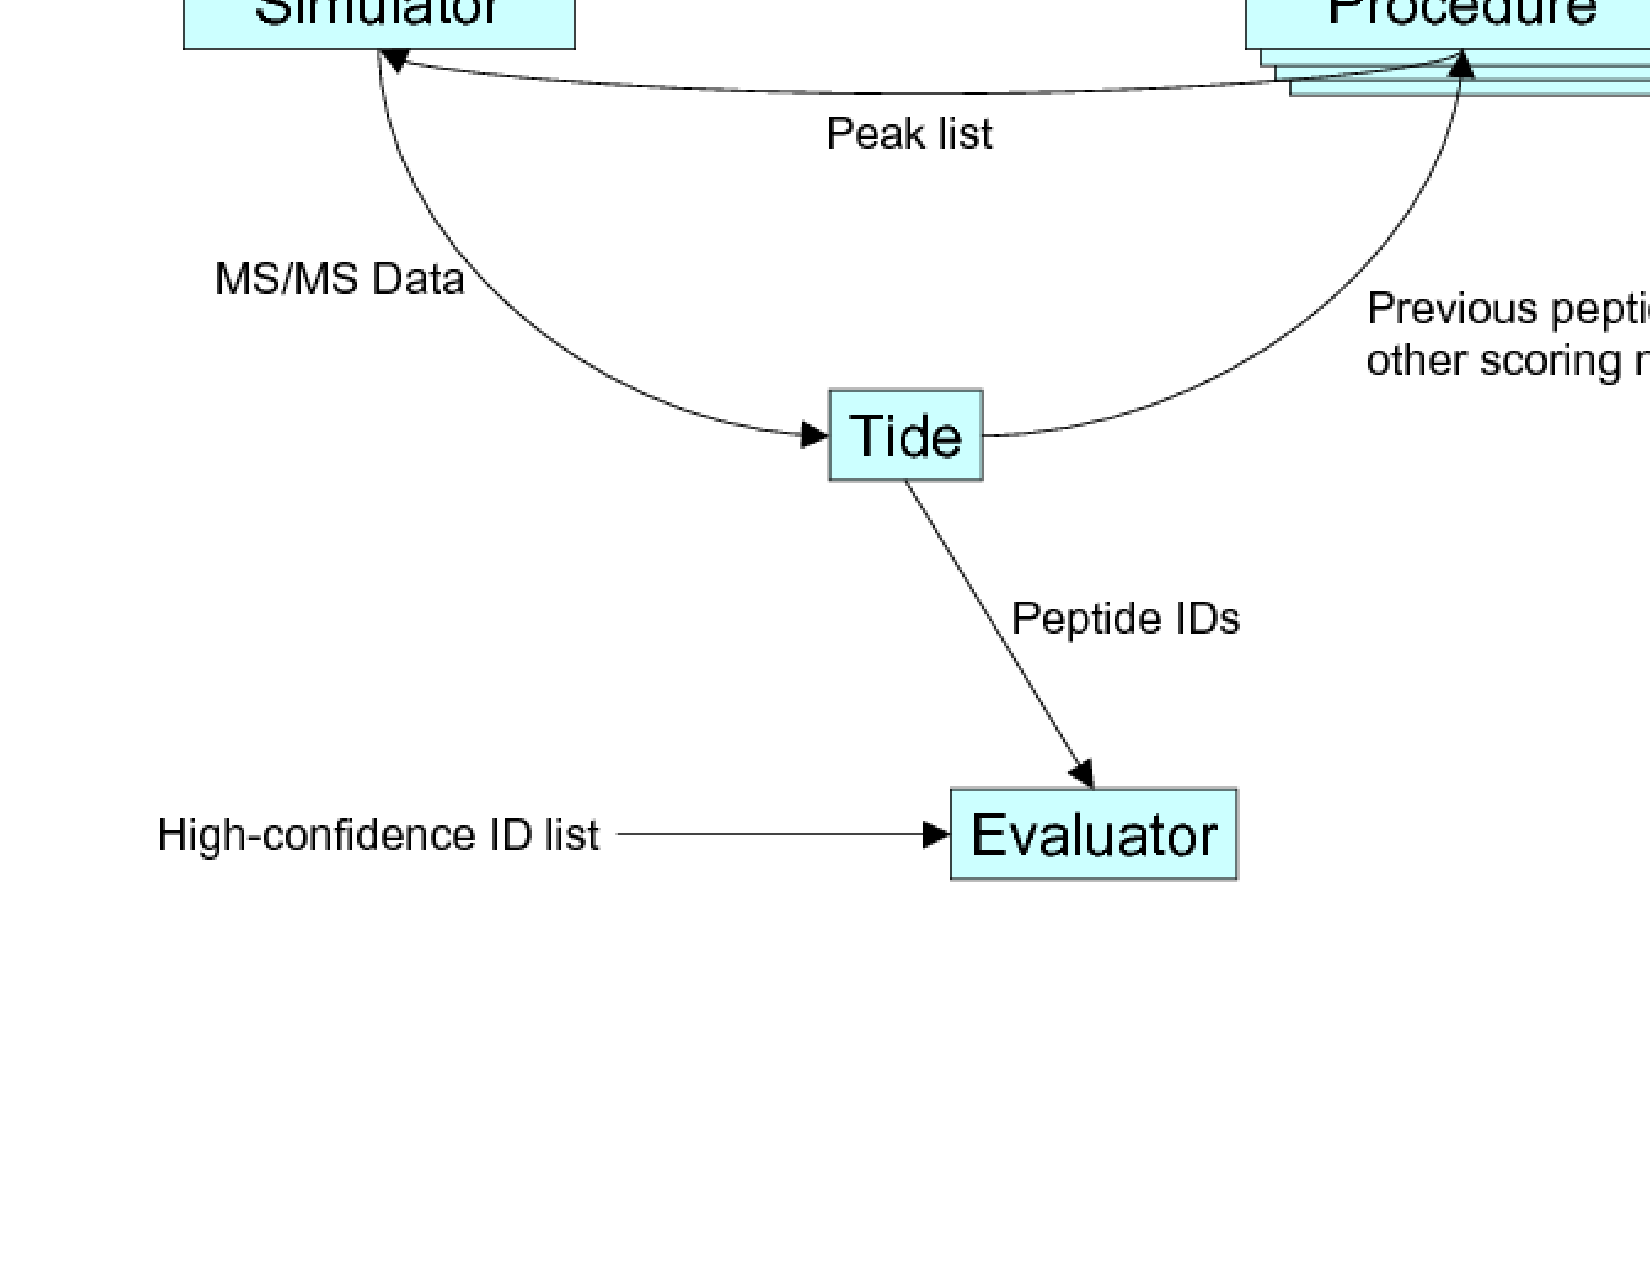
\includegraphics[width=6.0in]{SimulationFlow.pdf}
\caption[Structure of Spectrometer Simulator] {{\bf Structure of Spectrometer
    Simulator} The spectrometer simulator component runs through all the MS1
  scans from experiment e10, one at a time. It passes this MS1 data to a modular
  peak selection procedure, which selects peaks for fragmentation. The simulator
  checks whether it has a corresponding MS/MS scan. If it does, then it uses
  Tide to retrieve the corresponding identification and $\XCorr$ values. The
  information from Tide is also passed to the peak selection procedure. Finally,
  the list of identified peptides is sent to the evaluator for comparison
  against a precomputed list of high-confidence identifications.
  \label{figure:simulator}}
\end{figure}

We implemented in Python a framework for simulation according to the
diagram. The spectrometer simulator, the Tide results module, and the evaluator
were implemented in one Python program which was allowed to run with any
separately-supplied peak picker procedure. This enabled us to run thousands of
simulations under varying parameter settings.

\subsection{Simulation Data} %%4
\label{subsection:simulationdata}

In a perfect simulation, MS/MS scans would be available for any MS1 peak that a
peak selection algorithm might choose. In order to ensure a reasonable
simulation, we used a single MS1 experiment along with corresponding MS/MS
spectra from several replicate experiments.

The replicate experiments were taken from PAnDA data \cite{hoopmann:post}, a
collection of 11 experiments in total, of which six were ordinary replicates and
five were the result of preloading the spectrometer's exclusion list with the
accumulated list of peaks that were picked in replicates that had run
previously. The PAnDA paper concluded that more peptides were identifiable using
this method. Our hope was that this data would supply a diverse set of peaks to
the simulator that would be available to any given peak selection procedure. As
it turned out, there were still frequently peaks requested by a peak selection
procedure for which the simulator could not supply data. We discuss in the
evaluation metrics (Section~\ref{subsection:evalmetric}) how we handled this
problem.

We aligned the data from these replicate experiments by retention time. One
experiment, called {\it e10}, was used as the basis for MS1 data that the
simulator would give to the candidate peak picker. Then the MS/MS data was
taken from each of the other 10 experiments and compared with the MS/MS data of
e10. See Figure~\ref{figure:alignment}, which shows the computed retention-time
alignment between e10 and another replicate, e12, as an example. The aligned
points are shown in the scatter plot. We draw the retention times in the two
experiments of any MS/MS scan that was identified as the same peptide in both
experiments with 90\% confidence.

\begin{figure}
\centering
\includegraphics[width=6.0in]{e10-vs-e12.png}
\caption[Retention-time alignment of replicate experiments]{{\bf Retention-time
    alignment of replicate experiments} e10 and e12. We need to assign as many
  MS/MS scans as possible to the MS1 peaks from e10. This computation is the
  basis for using MS/MS data from another experiment (such as e12) to provide
  additional simulation information. We plot the retention times as green points
  where the two experiments gave identical identifications of MS/MS scans at
  90\% confidence. Then we fit a line so that the e12 data can be recast in
  terms of e10 retention times.
  \label{figure:alignment}}
\end{figure}

The MS1 data from e10, taken together with the aligned MS/MS data from all 11
experiments, forms the simulation data. Figure~\ref{figure:combinedmsms} shows
the result graphically: MS1 data from experiment e10 is interleaved with MS/MS
data from all replicates. The hope is that if a candidate peak picker requests
an MS/MS scan of a particular peak and it wasn't selected in the actual run of
e10, then one of the other experiments may have taken a scan of the same peak at
about the same time.

\begin{figure}
\centering
\includegraphics[width=6.0in]{combinedmsms.pdf}
\caption[MS1 data interleaved with combined MS/MS data from multiple
  experiments]{{\bf MS1 data interleaved with combined MS/MS data} from multiple
  experiments. A tiny region of the total data is shown magnified (about 7
  seconds and 2 $m/z$ from experiment e10, which ran 100 minutes and covered
  1000 $m/z$). The vertical red lines represent the MS1 data from experiment
  e10, with higher-intensity peaks indicated in brighter shades of red. A green
  tick mark shows peaks picked for analysis during the actual run of e10. A
  yellow tick mark shows where interpolated MS/MS data from another replicate
  experiment is available during simulation. In many cases, but not always,
  intense MS1 peaks have corresponding MS/MS data from one of the experiments.
  \label{figure:combinedmsms}}
\end{figure}

\subsection{Evaluation Metrics} \label{subsection:evalmetric}

The main metric we are interested in is the total number of unique peptides
identified over the course of the entire spectrometry experiment. However,
because of the limits inherent in simulation -- in particular, the simulator's
inability to return every MS/MS spectrum demanded -- we could not use this
simple metric to make reasonable comparisons against the basic exclusion list,
for which complete corresponding MS/MS data is available.

We therefore selected a two-dimensional metric: for a given experiment, we
assign a score by plotting a point in two dimensions. See
Figure~\ref{figure:baseline} for an example. On the $y$-axis we plot the number
of unique peptides identified. On the $x$-axis, we plot the number of spectrum
requests that were honored by the simulation (i.e. for which an MS/MS scan was
available). The two-dimensional metric enables us to look at a simulation
experiment and judge whether a greater or lesser number of peptide IDs can be
accounted for by a significant difference in the quality of the simulation, as
measured by the number of spectra successfully returned.

\section{Results} %%5

In investigating the utility of ID-informed peak selection, we examined several
approaches to peak picking. Each approach was aimed at achieving a provably
better rate of peptide identification than the basic exclusion list over the
course of a simulated mass spectrometry run.

To measure the peak-selection approaches systematically, we considered three
primary approaches with varying parameters. All methods we tried started with a
basic exclusion list implementation and proceeded from there with modifications
to the basic behavior. In an effort to match as closely as possible the behavior
of the spectrometer's on-board computer, we used the same exclusion list
settings in our experiments. The basic settings were:
\begin{itemize}
\item Exclusion duration: $18$ seconds ($0.3$ minutes).
\item Exclusion window: $\Delta m/z \in [-0.5, 1.5]$ relative to any excluded peak.
\end{itemize}
That is, when a candidate peak is considered for fragmentation, it is checked
for two criteria against every other peak previously chosen: if the candidate
occurs within 18 seconds of a previously chosen peak and also falls within the
exclusion window of that peak by $m/z$, then the candidate may not be picked. A
picture of these settings can be drawn by plotting the differences between all
pairs of selected peaks within e10, by precursor $m/z$ and retention time
(Figure~\ref{figure:deltas}). Such a picture is symmetric by construction, and
the blank region highlights the excluded differences. This picture shows that
our settings for the exclusion window and exclusion duration are correct.

\begin{figure}
\centering
\includegraphics[width=6.0in]{margins.png}
\caption[Pairwise differences between peaks in e10]{{\bf Pairwise differences
    between peaks in e10.} Shown are the differences in retention time and $m/z$
  between all pairs of nearby peaks that were actually selected for
  fragmentation in experiment e10. This illustrates the effect of the on-board
  exclusion list. We can see the $0.3$-minute retention time exclusion and the
  $[-0.5, 1.5]$ asymmetric $m/z$ exclusion window.
  \label{figure:deltas}}
\end{figure}

As a baseline for comparison of candidate peak-selection methods, we used a
simulation of the basic peak-selection protocol. This was done in order to
evaluate the performance of these experimental peak-selection methods
fairly. Figure~\ref{figure:baseline} shows the performance of the baseline
simulated exclusion list under various parameter settings.  The
parameterizations describe the tolerance of the simulator for returning MS/MS
data whose retention time or $m/z$ precursor differed from that requested.  In
Section~\ref{subsection:stability}, we discuss the question of the difficulty
and desirability of perfectly replicating the on-board computer's
peak-selection protocol.

\begin{figure}
\centering
\includegraphics[width=6.0in]{1_excl2.png}
\caption[Baseline performance of simulated exclusion list]{{\bf Baseline
    performance of simulated exclusion list.} Each plotted point represents a
  complete simulated mass spectrometry experiment under varying
  parameterizations (simulation tolerances). We plot the absolute number of
  peptides identified vs. the number of attempted peaks for which there was
  simulation data. The point in the upper right represents the actual e10
  experiment. The line represents the ratio of identifications to total peaks
  acquired throughout the run of e10.
  \label{figure:baseline}}
\end{figure}

Modulo parameterization, there were three peak-selection methods we implemented,
detailed in the following sections, each with performance evaluations. In all
results, we ran the experiment multiple times, varying the simulation
tolerances. We describe the peak-selection methods and show diagrammatic results
in the following sections.

\subsection{Variable-Duration Exclusion List}

The hypothesis of our first peak-picking method was that a peak is that the
basic exclusion list duration is not optimal for acquiring a diversity of
peptides, once the peptides are knowable. The 18-second exclusion list duration
is essentially a compromise. Peaks corresponding to quickly-eluting peptides
should come off the list quickly to make room for another peptide species to
begin eluting. Peaks corresponding to slowly-eluting peptides should remain on
the list until they are past. However, if you can know the identity of the
selected peaks, a repeated identification is a good indication that the peptide
is still eluting. In that case, a longer than normal exclusion list duration
should apply for that peak.

In order to implement this strategy, we gather peaks in order of intensity, just
as for the basic exclusion list, but we modify the decision to include or
exclude them. We allow a peak to be requeried after the normal
exclusion time. However, if a peak is requeried and is identified as the same
peptide as previously, the peak subsequently remains on the exclusion list for
three times longer.

The results are shown in Figure~\ref{figure:variable}. We can see that for a
majority of simulation settings (most individual plotted points), the variable
exclusion list gives slightly more peptide IDs than the simulated basic
exclusion list. However, the difference in performance is extremely modest: an
average increase of 1.9 distinct peptide IDs out of an average total of 997 for
the basic exclusion list.

\begin{figure}
\centering
\begin{tabular}{cc}
\includegraphics[width=3.0in]{2_variable2.png} &
\includegraphics[width=3.0in]{2b_variable2.png} \\
Identifications & Deltas \\
\end{tabular}
\caption[Evaluation of the Variable-Duration Exclusion List peak selector]{{\bf
    Evaluation of the Variable-Duration Exclusion List peak selector.}  The left
  panel shows the results of simulations, under varying tolerances, of the
  variable exclusion list peak selection procedure (see text). We also repeat
  the results for the basic exclusion list (Figure~\ref{figure:baseline}) as a
  basis for comparison. As in Figure~\ref{figure:baseline}, we plot the absolute
  number of peptides identified vs. the number of attempted peaks for which
  there was simulation data. On the right panel, for each setting of simulation
  tolerances, we plot the result differences between the variable exclusion list
  and the basic exclusion list. The $y$-axis shows the difference in the number
  of unique peptide IDs and the $x$-axis shows the difference in the number of
  selected peaks for which simulation data was available.
  \label{figure:variable}}
\end{figure}

\subsection{Weibull-score Triage}

The second peak-picking method we investigated is based on the hypothesis that
if a peak is not confidently identified, this may be due to noise, and a second
attempt may enable a more confident identification on the second try (probably
with the same result as before). On the other hand, if a peak yields a poor
spectrum, then there is no point in retrying, as a new attempt is likely to give
the same difficulties.

This hypothesis sets up a natural triage as follows. If a peak is identified
with high confidence or low confidence, then it should be placed on the
exclusion list according to the standard protocol. If the peak is identified
with middling confidence, then we allow it to be requeried after a much shorter
interval.

We used the confidence estimation metric introduced in Crux \cite{park:rapid},
based on fitting a Weibull curve to the tail of the scoring distribution over
the candidate peptides. We allowed this on the theory that if this method worked
well, we could introduce the Weibull-based confidence estimator into Tide while
keeping the performance high enough to meet the throughput and latency
requirements for real-time peptide identification.

We applied the following specific protocol:
\begin{enumerate}
\item If a selected peak was identified with a $p$-value of $0.01$
according to the Weibull curve fit, then it was placed on the exclusion list
normally.
\item If a selected peak failed to be identified confidently ($p$-value $>0.1$),
  then it was also placed on the exclusion list normally.
\item If a selected peak was identified with intermediate confidence ($p$-value
  between $0.01$ and $0.1$), then it was placed on the exclusion list {\em only
    briefly} and was allowed to be requeried after 5 seconds.
\end{enumerate}

This approach performed noticeably poorly relative to the basic exclusion list
-- about 19\% fewer identifications than the basic exclusion list, averaged
across a variety of tolerances, albeit with 11\% fewer available simulation
peaks. Detailed results are shown in Figure~\ref{figure:triage}. Since this
approach performed poorly, we do not show the results of attempting other triage
thresholds.

\begin{figure}
\centering
\begin{tabular}{cc}
\includegraphics[width=3.0in]{3_weib_triage2.png} &
\includegraphics[width=3.0in]{3b_weib_triage2.png} \\
Identifications & Deltas \\
\end{tabular}
\caption[Evaluation of the Weibull-Triage peak selector]{{\bf Evaluation of the
    Weibull-Triage peak selector.}  The left panel shows the results of
  simulations, under varying tolerances, of the Weibull-triage peak selection
  procedure (see text). We also repeat the results for the basic exclusion list
  (Figure~\ref{figure:baseline}) as a basis for comparison. As in
  Figures~\ref{figure:baseline} and \ref{figure:variable}, we plot the absolute
  number of peptides identified vs. the number of attempted peaks for which
  there was simulation data. On the right panel, for each setting of simulation
  tolerances, we plot the result differences between the Weibull-triage method
  and the basic exclusion list. The $y$-axis shows the difference in the number
  of unique peptide IDs and the $x$-axis shows the difference in the number of
  selected peaks for which simulation data was available.
  \label{figure:triage}}
\end{figure}

\subsection{Charge state exclusion}

The third peak-picking method we investigated is based on the fact that the same
peptide may elute roughly simultaneously at two different charge states. The
basic peak selection protocol may then end up choosing both such peaks. No
effort is made to prefer one over the other, because it may be easier to
identify the peptide at one charge state or the other, and the spectrometer does
not know {\it a priori} which is preferable.

However, we may hypothesize that if a peak is identified with high confidence at
one charge state, then we can reasonably exclude the corresponding peaks at the
other charge states as well, because they are likely to be the same peptide
species. If a peak is not identified with high confidence, then it may be
treated as before.

The results, shown in Figure~\ref{figure:chargestate}, are somewhat more
promising than for the other peak picking methods we examined, but remain
modest: an average of 10 more unique peptide identifications (1\%) over the
simulated basic exclusion list. To be sure of the effect, we also show the
results (shown in red crosses) of simply excluding peaks at sister charge states
on a first-come-first-served basis, without regard to whether the identification
at the first attempted charge state was made confidently. These results are
worse than the basic exclusion list and show that real-time identification was
critical in gaining the additional identifications seen in the charge state
exclusion method.

\begin{figure}
\centering
\begin{tabular}{cc}
\includegraphics[width=3.0in]{4_chargestates2.png} &
\includegraphics[width=3.0in]{4b_chargestates2.png} \\
Identifications & Deltas \\
\end{tabular}
\caption[Evaluation of the Charge-State Exclusion peak selector]{{\bf Evaluation
    of the Charge-State Exclusion peak selector.} As in
  Figures~\ref{figure:baseline}--\ref{figure:triage}, the left panel shows the
  results of simulations, under varying tolerances, of the charge-state
  exclusion peak selection procedure (see text).  For comparison, we also
  plotted (red crosses) the results of excluding charge-state sister peaks
  without benefit of acquiring the peptide IDs in real time.  On the right
  panel, as in Figures~\ref{figure:baseline}--\ref{figure:triage}, for each
  setting of simulation tolerances, we plot the result differences between the
  charge-state exclusion method and the basic exclusion list.
  \label{figure:chargestate}}
\end{figure}

To aid in visualizing the different effects of the three methods we tried, we
show the combined results of all experiments in Figure~\ref{figure:all}. There
we can see that the Weibull-triage method fared poorly, while the other two
methods showed very slight improvements over the basic exclusion list, with the
charge-state exclusion being the most promising.

\begin{figure}
\centering
\begin{tabular}{cc}
\includegraphics[width=3.0in]{5_all2.png} &
\includegraphics[width=3.0in]{5b_all2.png} \\
Identifications & Deltas \\
\end{tabular}
\caption[Combined view of results from all IDIPS experiments]{{\bf Combined view
    of results from all IDIPS experiments.} As in
  Figures~\ref{figure:baseline}--\ref{figure:chargestate}, the left panel shows
  the results of simulations, under varying tolerances, of the various peak
  selection procedures as well as the simulated basic exclusion list.  On the
  right panel, as in Figures~\ref{figure:baseline}--\ref{figure:chargestate},
  for each setting of simulation tolerances, we plot the result differences
  between the experimental peak selection methods and the basic exclusion list.
  \label{figure:all}}
\end{figure}


\subsection{Remarks on the Operation of the Exclusion List}
\label{subsection:stability}

We drew three general observations regarding the operation of the on-board
computer's exclusion list, which affected all of the peak selection strategies
we attempted, and which were not obvious {\it a priori}.

The first observation about the on-board computer's exclusion list is that peaks
that are selected for fragmentation are often not taken from the top few peaks
by intensity. Rather, because of the exclusion list, and probably because the
actual spectrometer's peak selection algorithm includes some features of which
we were not aware, peaks of relatively low intensity are frequently
selected. Some of these peaks had intensities that ranked below hundreds of
other peaks in the same MS1 scan.

The second general observation is that some very intense peaks are often
excluded by the basic method. Often, a dozen or so peaks of high intensity are
completely skipped each minute of the experiment. This happens either as a
direct effect of the exclusion list or possibly because a more sophisticated
approach is used by the spectrometer to choose only one peak from each isotope
series.

The third general observation is that the exclusion list is surprisingly
unstable in that slight perturbations in the choice of peaks early in the
experiment lead to more far-reaching differences in the choice of peaks later
on. This phenomenon appears to be the result of a feedback effect between the
peak-selector and the exclusion list over the course of a run: a change in peak
leads to a different exclusion list, which leads to a subsequent change in peak,
and so on. This third effect is further magnified by the first two.

Together these effects contribute to the difficulty of simulating the
spectrometer's operation: peaks requested by a candidate peak-selection
mechanism may not be available, despite our use of data from replicate
experiments.

We note furthermore that the instability of the exclusion list argues against
attempting to replicate exactly the mechanism of the on-board peak selector.
Experimental peak selectors will necessarily deviate from the on-board peak
selector's choices, so the subsequent effects of exclusion list instability are
unavoidable in evaluating alternative peak selectors. It therefore makes sense
in evaluation to use a baseline that is subject to the same instability.

\section{Conclusions}

This section of the thesis described peptide identification in real time, and
ID-informed peak selection in the context of data dependent acquisition.  We
showed in Section~\ref{section:lowlatency} that with Tide's speed, it is
possible to analyze and identify peptides in real time as they are acquired by
the spectrometer. Accommodation would have to be made for the fact that Tide
currently processes spectra as a batch, but we showed that this limitation could
be overcome to create a very low latency version of Tide. This would be a
prerequisite for IDIPS.

We then implemented a spectrometer simulator together with several IDIPS
strategies, in hopes of showing that more peptides could be identified in the
course of an LC-MS/MS experiment if we had access to the identity of the
previously acquired peptides along the way. We developed three peak-selection
strategies to take specific advantage of low-latency peptide identification.

The results, however, were very modest at best: we could not, using a
simulation, demonstrate that any of the three peak-selection strategies would
yield more than a 1\% increase in unique peptide identifications than the
standard exclusion list or would likely outperform simpler methods that
considered only MS1 data.

From analyzing the peak-selection strategies we tried, it seems that the
better-performing approaches rely on aggressively excluding peaks rather than
relaxing the exclusion criteria. Rather than requerying peaks that failed to be
identified previously, we are better off excluding those peaks that have any
likelihood of being a duplicate. Our interpretation is that this is because the
generally low identification rate of peptides is a stronger effect than that of
noise in the spectrum.

We were stymied in getting positive results by at least four effects. The first
was the insufficiency of data for a good simulation: many requested peaks did
not have corresponding scans. The second was that results were more
sensitive to uninteresting parameters than interesting ones, such as simulation
tolerances. The third is that only a minority of spectra ever get confidently
identified, even without the limitations imposed by speed and latency
requirements. The fourth is that the actual peak-picking strategy employed by
the spectrometer is apparently more complex than a straightforward exclusion
list.

We attempted to overcome the inadequacy of simulation and sensitivity to
uninteresting parameters in three ways. First, we used lots of replicate
experimental data, including data specifically intended to expand peak
coverage. Second, we allowed the simulation tolerances and exclusion list
parameters to vary, and we aggregated over all of those results. Third, we
applied a two-dimensional success metric that attempts to correct for missing
simulation data.

We addressed the difficulty of getting confident identifications in two
ways. First, we allowed candidate peak-picking strategies access to quality
metrics, which we employed in the triage peak selection method and the charge
state exclusion method. Second, we tried several distinct peak-picking
strategies.

We were able to show a modest gain (1\%) in the number of peptides identified
using real-time peptide identification using one of the new peak-selection
procedures we investigated. While further improvement may be possible by more
complicated means, we have exhausted all the simple measures we set out to try
through simulation. We therefore conclude that proving a clear benefit from
real-time peptide identification will require significant further investigation.

\cleardoublepage
\section*{Acknowledgments}

The authors wish to thank Charles Grant, Barbara Frewen, Larry Ruzzo, Jimmy Eng,
and Mike MacCoss for useful conversations, and Sean McIlwain for help in the
design of the benchmarking scripts used to track running times of program
runs. The latest version of Tide also benefits greatly from the contributions of
Eva Baker, who implemented the output formatting program for Tide.  This work
was supported by NIH awards R01~EB007057 and T32~HG00035.

\bibliographystyle{unsrt}
\bibliography{refs}

\end{document}
